\documentclass[a4paper,14pt]{article}

\usepackage{comment} % Para comentar várias linhas ao mesmo tempo

%matemática
\usepackage{amsmath}
\usepackage{amssymb}

%diagramação
\usepackage{extsizes}
\everymath{\displaystyle}
\usepackage{geometry}
\usepackage{fancyhdr}
\usepackage{multicol}
\usepackage{graphicx}
\usepackage[brazil]{babel}
\usepackage[shortlabels]{enumitem}
\usepackage{cancel}
\usepackage{textcomp}
\usepackage{tcolorbox}

%tabelas
\usepackage{array} % Para melhor formatação de tabelas
\usepackage{longtable}
\usepackage{booktabs}  % Para linhas horizontais mais bonitas
\usepackage{float}   % Para usar o modificador [H]
\usepackage{caption} % Para usar legendas em tabelas
\usepackage{wrapfig} % Para usar tabelas e figuras flutuantes


%tikzpicture
\begin{comment}
	\usepackage{tikz}
	\usepackage{scalerel}
	\usepackage{pict2e}
	\usepackage{tkz-euclide}
	\usetikzlibrary{calc}
	\usetikzlibrary{patterns,arrows.meta}
	\usetikzlibrary{shadows}
	\usetikzlibrary{external}
\end{comment}


%pgfplots
\usepackage{pgfplots}
\pgfplotsset{compat=newest}
\usepgfplotslibrary{statistics}
\usepgfplotslibrary{fillbetween}

%colours
\usepackage{xcolor}



\columnsep=2cm
\hoffset=0cm
\textwidth=8cm
\setlength{\columnseprule}{.1pt}
\setlength{\columnsep}{2cm}
\renewcommand{\headrulewidth}{0pt}
\geometry{top=1in, bottom=1in, left=0.7in, right=0.5in}

\pagestyle{fancy}
\fancyhf{}
\fancyfoot[C]{\thepage}

\begin{document}
	
	\noindent\textbf{6FMA10 - Matemática} 
	
	\begin{center}Frações e decimais (Versão estudante)
	\end{center}
	
	\noindent\textbf{Nome:} \underline{\hspace{10cm}}
	\noindent\textbf{Data:} \underline{\hspace{4cm}}
	
	%\section*{Questões de Matemática}
	
	\begin{multicols}{2}
		\noindent Podemos representar uma fração por um numeral decimal. Por exemplo, $\frac{1}{10}$ pode ser escrito como 0,1 (lê-se "um décimo" ou "zero vírgula um"). \\
		\noindent\textsubscript{-----------------------------------------------------------------------}
		\begin{enumerate} 
			\item Com base no que você viu em aula, tente escrever cada uma das frações abaixo como numerais decimais.
			\begin{enumerate}[a)]
				\item $\frac{2}{10} = $ \\\\\\\\\\
				\item $\frac{5}{10} = $ \\\\\\\\\\
				\item $\frac{9}{10} = $ \\\\\\\\\\
				\item $\frac{7}{10} = $ \\\\\\
				\item $\frac{8}{10} = $ \\\\\\\\\\
				\item $\frac{6}{10} = $ \\\\\\\\\\
			\end{enumerate}
			\item Escreva como se lê $\frac{3}{10}$. \\\\\\\\\\
			\item Escreva como se lê 0,4. \\\\\\\\\\
			\item Mário tem seis décimos da idade de Rafael. Rafael tem cinco décimos da idade de Eduardo, que tem 40 anos. Quantos anos tem Mário? \\\\\\
			%37 a 39
			\item Miguel tem $\frac{1}{6}$ da idade de seu pai, que tem 42 anos. Mariana tem $\frac{1}{4}$ da idade de sua mãe, que tem 32 anos. Quem é mais velho: Miguel ou Mariana? \\\\\\\\\\\\\\\\\\\\
			\item Durante um jogo de tênis, $\frac{4}{9}$ das bolas foram perdidas. Sabe-se que, para este jogo, foram utilizadas 27 bolas. Com base nessas informações:
			\begin{enumerate}[a)]
				\item quantas bolas se perderam? \\\\\\\\\\\\\\
				\item quantas bolas restaram? \\\\\\\\\\\\\\
				\item desenhe as bolas que restaram no espaço a seguir. \\
				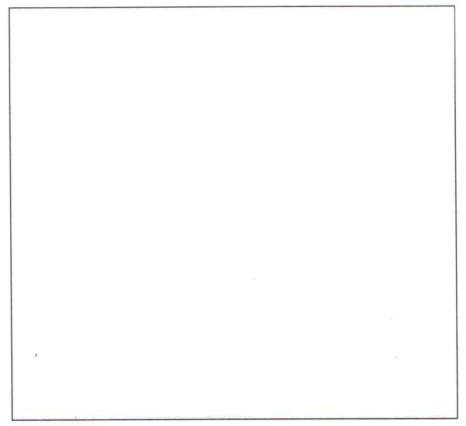
\includegraphics[width=1\linewidth]{6FMA10_imagens/imagem1}
				\item No $shopping$ de uma cidade foi montada uma piscina com 12 000 bolinhas para crianças de 1 a 4 anos. No fim da manhã, $\frac{4}{15}$ das bolinhas estavam fora da piscina. O instrutor da atividade recolheu todas e não as colocou de volta. Durante a tarde, 3 300 bolinhas foram retiradas.
				\begin{enumerate}[a)]
					\item Quantas bolinhas restaram na piscina no fim da manhã? \\\\\\\\\\\\\\
					\item Que fração as bolinhas retiradas no período da tarde representam a quantidade de bolinhas que sobraram após o período da manhã? \\\\\\\\
				\end{enumerate}
			\end{enumerate}
		\end{enumerate}
	\end{multicols}
\end{document}